\section{多用户MIMO上行系统}
\subsection{基于AI的多用户MIMO检测}
\subsubsection{DeepSIC\cite{2020DeepSIC}}
\href{https://github.com/nirshlezinger1/DeepSIC}{源码} \par 
\paragraph{缺点}
文章只探究了固定信道的性能,且网络中没有利用信道矩阵H的信息,很难在时变信道情况下应用该网络,文章提到了在线训练的方法,但是该方法和我们研究的直接使用信道矩阵和接收信号进行检测有一定的差异性。
\paragraph{系统模型}
\begin{equation}
    y=Hx+n
\end{equation}
其中,$H_{i,j}=e^{-|i-j|},i\in \{1,\cdots,N_r\}, j\in \{1,\cdots, K\}$
\paragraph{核心思想}\par 
利用传统的迭代干扰消除的思想,每一次迭代将已检测出的信号当作干扰从接收信号中消除,然后检测剩下的符号。传统的干扰消除的消除方法是直接将其余估计信号从接收信号中减去,然后估计待估计信号。其原理如图所示: \par 
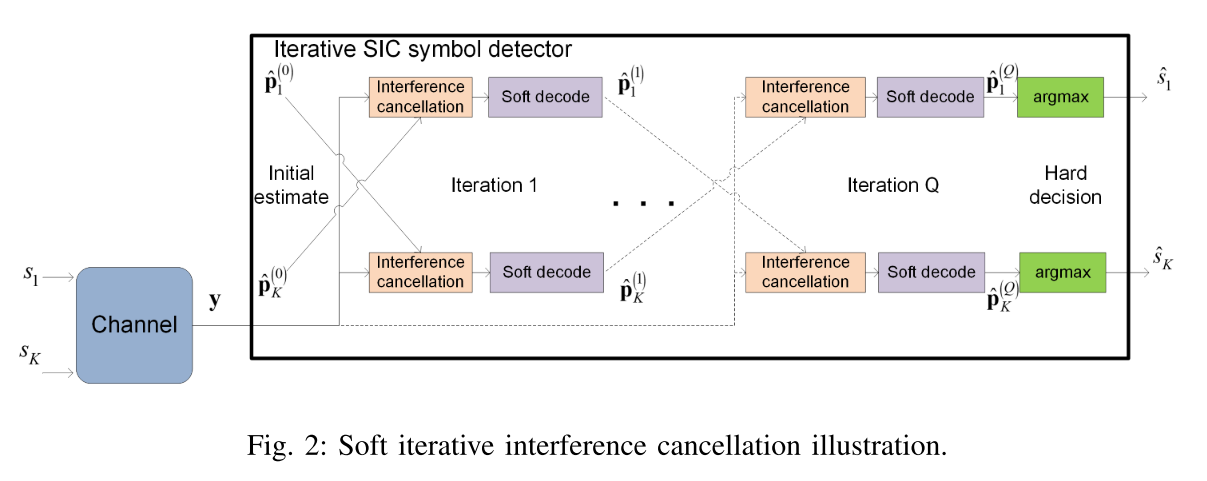
\includegraphics[width=0.99\textwidth]{SIIC.PNG}
% \begin{figure}[ht]
%     \centering
%     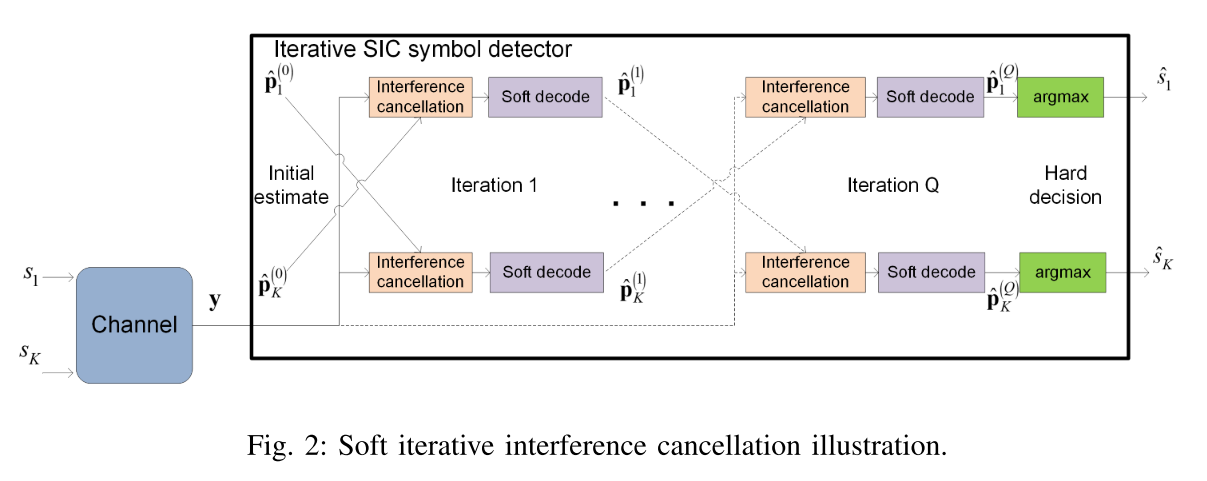
\includegraphics[width=0.99\textwidth]{SIIC.PNG}
% \end{figure}
因为传统的干扰消除模块有一定的局限性,一是将信道视为线性信道模型,不适用于非线性信道,二是需要获取信道矩阵以及信道噪声的准确信息。为了解决这个问题,文章提出将传统的干扰消除模块用一个DNN网络来代替,通过数据训练的方法获取最优的基于网络的干扰消除模块,将该网络称为DeepSIC。
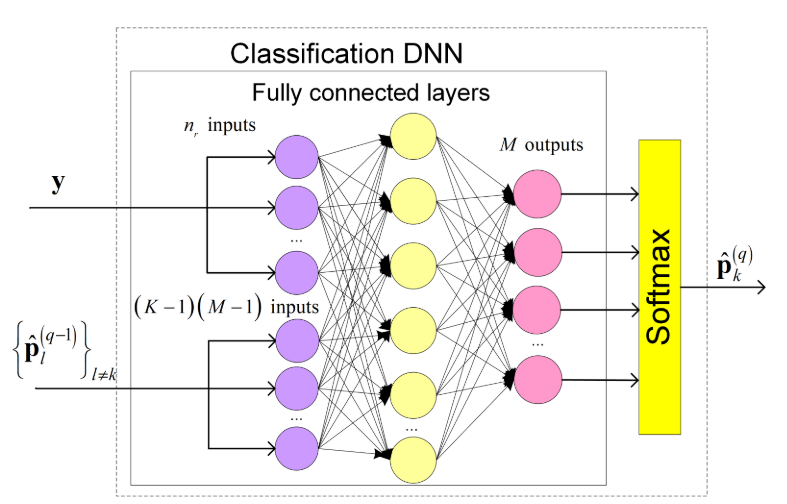
\includegraphics[width=0.9\textwidth]{分类DNN.PNG}
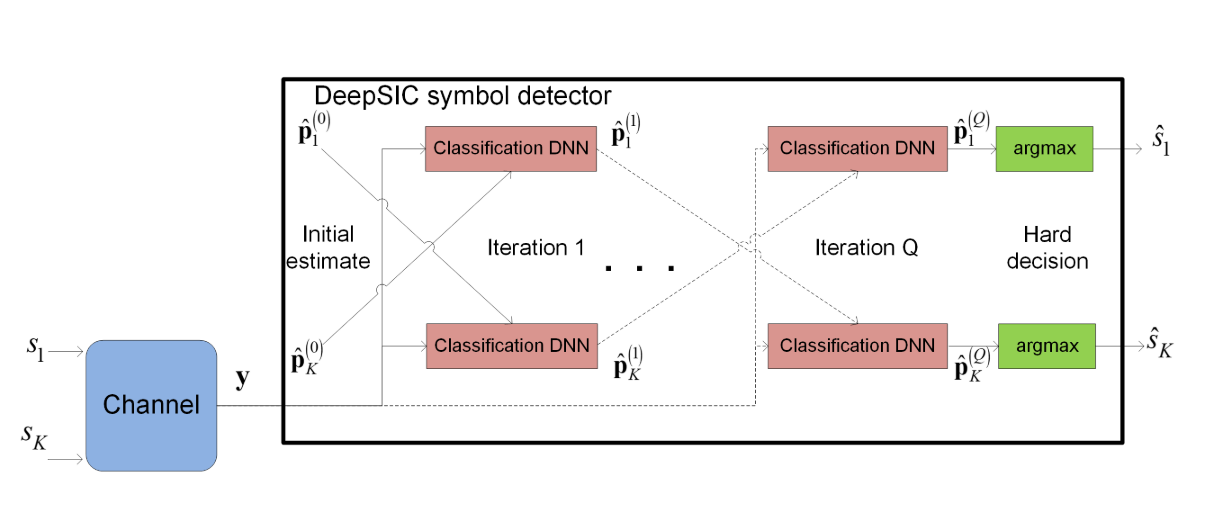
\includegraphics[width=0.9\textwidth]{DeepSIC框图.PNG}
\paragraph{损失函数}
\begin{equation}
    L_{SumCE}(\bm{\theta})=\frac{1}{n_t}\sum_{j=1}^{n_t}\sum_{k=1}^{K}-\log \hat{\bm{p}}_k^{(Q)}(\tilde{\bm{y}}_j,(\tilde{\bm{s}}_j)_k;\bm{\theta})
\end{equation}
\subsubsection{MLD+DCNN\cite{2020A}}
\paragraph{系统模型}
\begin{equation}
    \begin{aligned}
    \bm{y}(n)&=\bm{H}(n)\bm{s}(n)+\bm{w}(n) \\ 
    \bm{w}(n+1)&=\sqrt{\rho}\bm{w}(n)+\sqrt{1-\rho}\bm{u}(n+1)
    \end{aligned}
\end{equation}
\paragraph{核心思想} 
文章针对时域相关的噪声环境提出了MLD+DCNN的网络结构,其中MLD用于符号检测,DCNN用于噪声估计,通过MLD和DCNN结构将时域相关噪声解相关为时域不相关的噪声,从而使得MLD检测获得更优的性能。
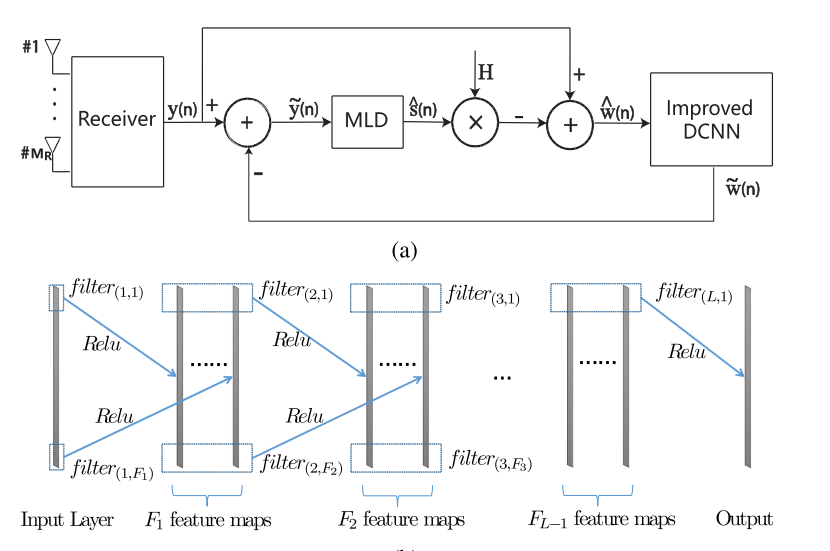
\includegraphics[width=0.9\textwidth]{MLD_DCNN.PNG}

\subsubsection{MMNet}
\subsubsection{OAMPNet}
\subsubsection{DetNet}

% \begin{figure}
%     \subfigure{
%         \centering
%         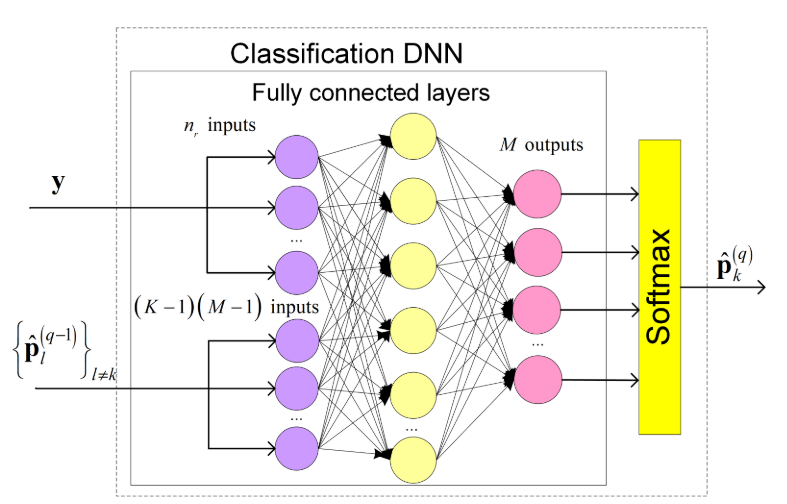
\includegraphics[width=0.9\textwidth]{分类DNN.PNG}
%         }
%     \subfigure{
%         \centering
%         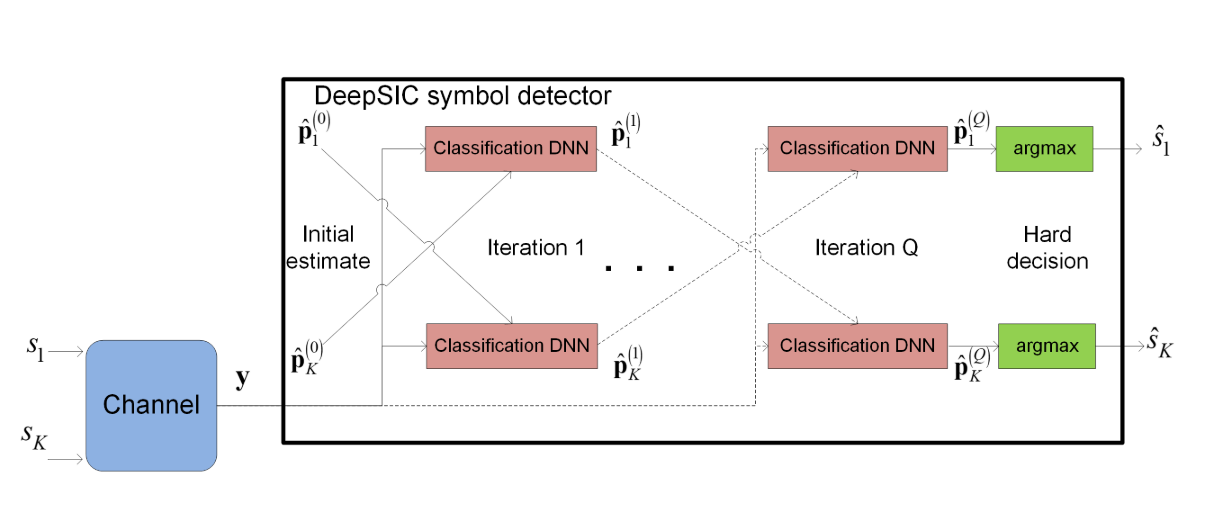
\includegraphics[width=0.9\textwidth]{DeepSIC框图.PNG}
%     }
% \end{figure}
% \begin{enumerate}
%     \item DeepSIC\cite{2020DeepSIC} \par 
%         系统模型$y=Hx+n$,$H_{i,j}=e^{-|i-j|},i\in \{1,\cdots,N_r\}, j\in \{1,\cdots, K\}$ \par 
%     \item 
% \end{enumerate}